\begin{figure}[htbp]
\centering
\resizebox{0.95\textwidth}{!}{%
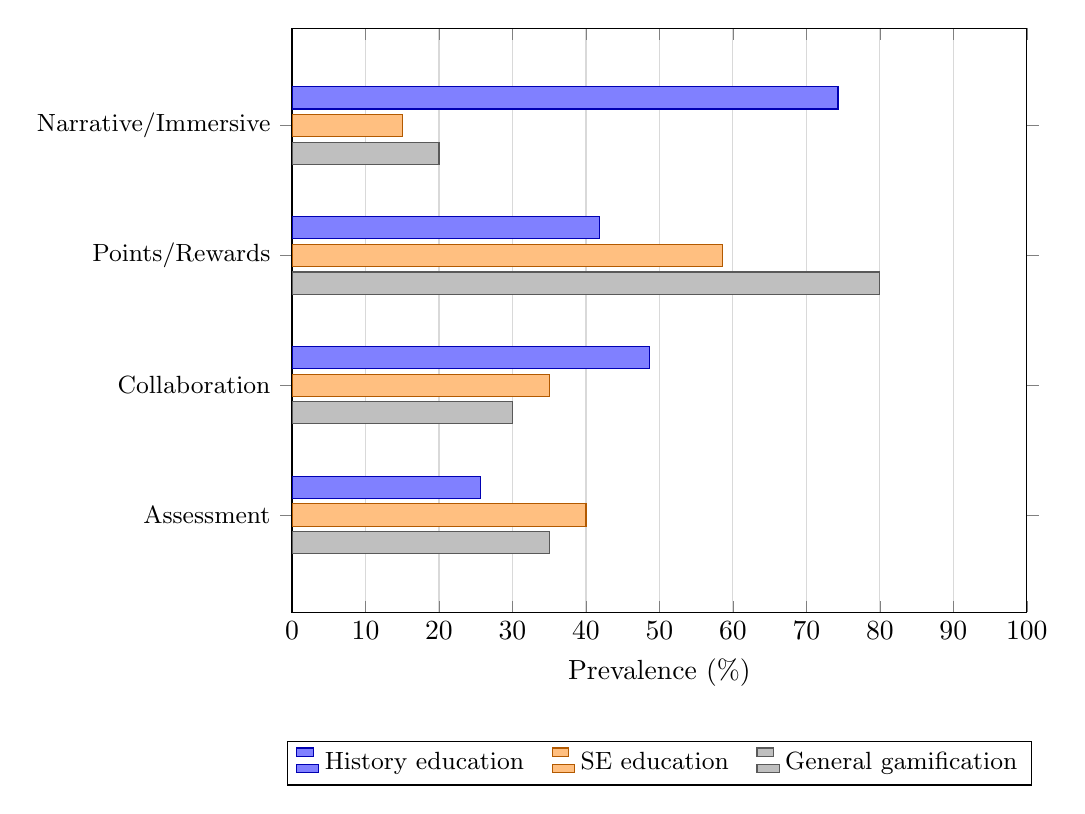
\begin{tikzpicture}
\begin{axis}[
    xbar,
    width=0.9\textwidth,
    height=9cm,
    xlabel={Prevalence (\%)},
    symbolic y coords={
      {Assessment},
      {Collaboration},
      {Points/Rewards},
      {Narrative/Immersive}
    },
    ytick=data,
    y tick label style={font=\small, anchor=east},
    bar width=8pt,
    xmin=0, xmax=100,
    enlarge y limits=0.25,
    xmajorgrids=true,
    ymajorgrids=false,
    grid style={gray!30},
    legend style={
      at={(0.5,-0.22)},
      anchor=north,
      legend columns=3,
      font=\small,
      /tikz/every even column/.append style={column sep=8pt},
    },
    reverse legend,
]
% General gamification (plotted first = bottom bar in each group)
\addplot[fill=gray!50, draw=gray!70!black] coordinates {
  (35,{Assessment})
  (30,{Collaboration})
  (80,{Points/Rewards})
  (20,{Narrative/Immersive})
};
% SE education
\addplot[fill=orange!50, draw=orange!70!black] coordinates {
  (40,{Assessment})
  (35,{Collaboration})
  (58.6,{Points/Rewards})
  (15,{Narrative/Immersive})
};
% History education (plotted last = top bar in each group)
\addplot[fill=blue!50, draw=blue!70!black] coordinates {
  (25.7,{Assessment})
  (48.6,{Collaboration})
  (41.9,{Points/Rewards})
  (74.3,{Narrative/Immersive})
};
\addlegendentry{General gamification}
\addlegendentry{SE education}
\addlegendentry{History education}
\end{axis}
\end{tikzpicture}%
}
\caption{Comparison of game design element prevalence across three educational domains. History education exhibits an inverted profile: experiential elements (narrative, immersion) dominate over reward elements (points), reversing the pattern observed in software engineering education and general gamification.}
\label{fig:domain-element-comparison}
\end{figure}
